\documentclass[aspectratio=169]{beamer}
\setbeamertemplate{navigation symbols}{}
\usepackage{color, amsmath, comment, subfigure}
\usepackage{url}

\usepackage{hyperref}
\hypersetup{
    colorlinks=true,
    linkcolor=blue,
    filecolor=magenta,      
    urlcolor=cyan,
}

%%%%%%%%%%%%%%%%%%%%%%%%%%
\title[]{Pre-read for Tuesday, October 20:\\Weather, Lorenz attractor}
\author[]{Matthew J. Salganik}
\institute[]{}
\date[]{COS 597E/SOC 555 Limits to prediction\\Fall 2020, Princeton University}

\begin{document}
%%%%%%%%%%%%%%%%%%%%%%%%%%%
\frame{\titlepage}
%%%%%%%%%%%%%%%%%%%%%%%%%%%
\begin{frame}
\frametitle{}

Interested in system that are not random but looks random.  Could also be said as systems that are deterministic but do not look deterministic.
\pause
\begin{itemize}
\item tumbling of a rock down a mountainside
\item breaking of waves on the shore
\end{itemize}

\pause
For our class these are interesting examples because
\begin{itemize}
\item there are precise laws governing behavior
\item they are unpredictable in some ways, but predictable in others
\end{itemize}

\end{frame}
%%%%%%%%%%%%%%%%%%%%%%%%%%%%%
\begin{frame}

sensitive dependence on initial conditions: two nearly identical initial conditions diverge until they bear not more resemblance than two states chosen randomly

\pause
\begin{itemize}
\item pinball machine
\pause
\item ski slope
\end{itemize}

\end{frame}
%%%%%%%%%%%%%%%%%%%%%%%%%%%%
\begin{frame}
\frametitle{}

\begin{center}
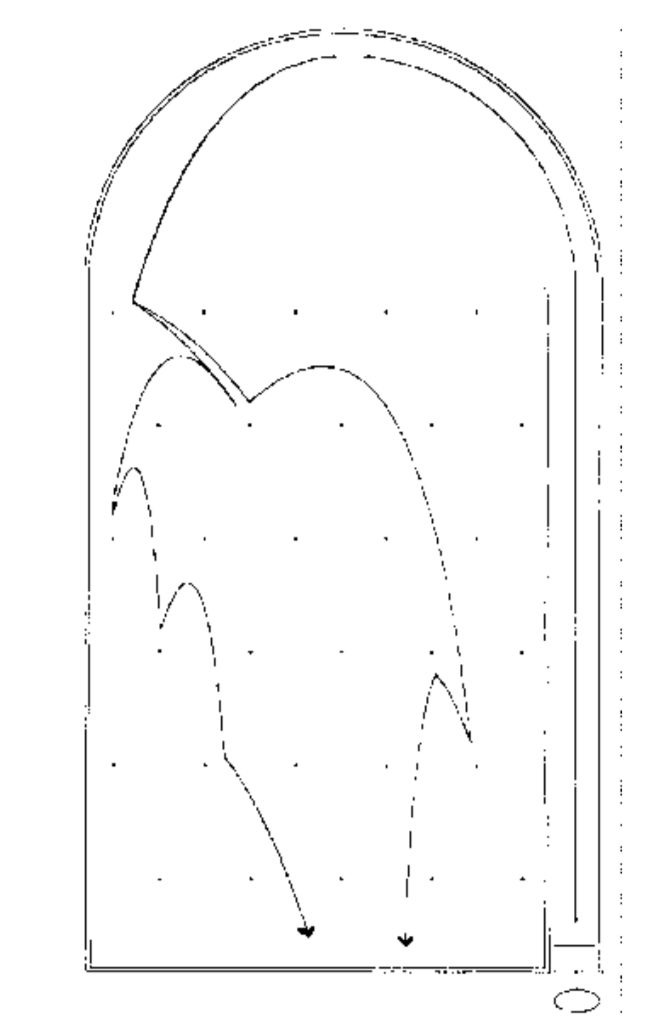
\includegraphics[height = 0.9\textheight]{figures/lorenz_essence_1993_fig1}
\end{center}

\end{frame}
%%%%%%%%%%%%%%%%%%%%%%%%%%%%%
\begin{frame}
\frametitle{}

\begin{center}
\only<1>{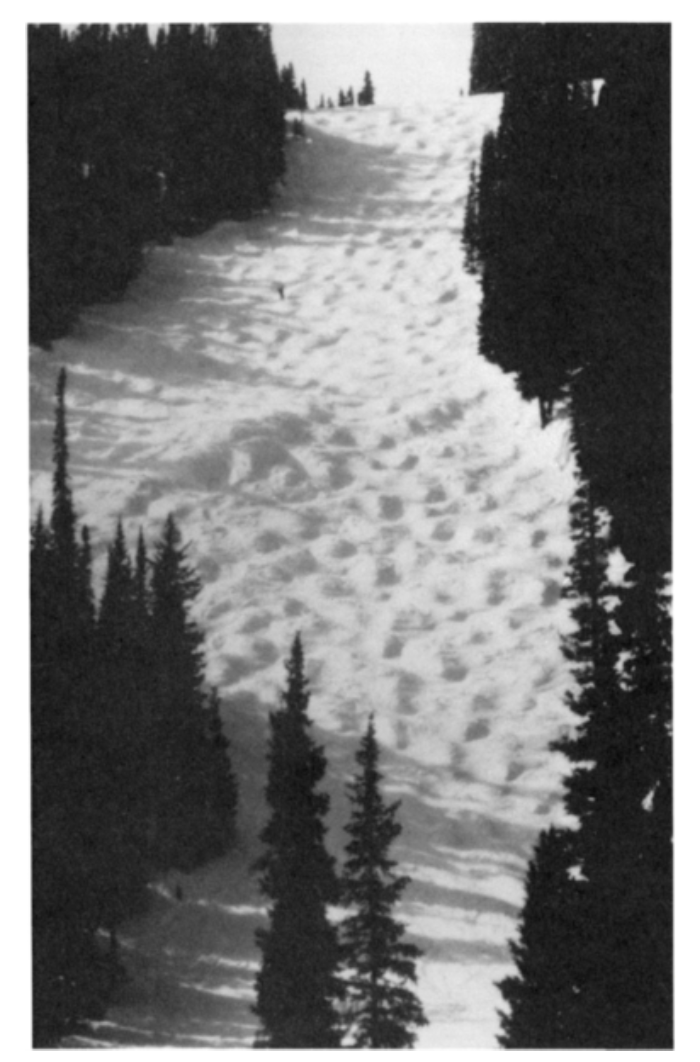
\includegraphics[height = 0.9\textheight]{figures/lorenz_essence_1993_fig5}}%
\only<2>{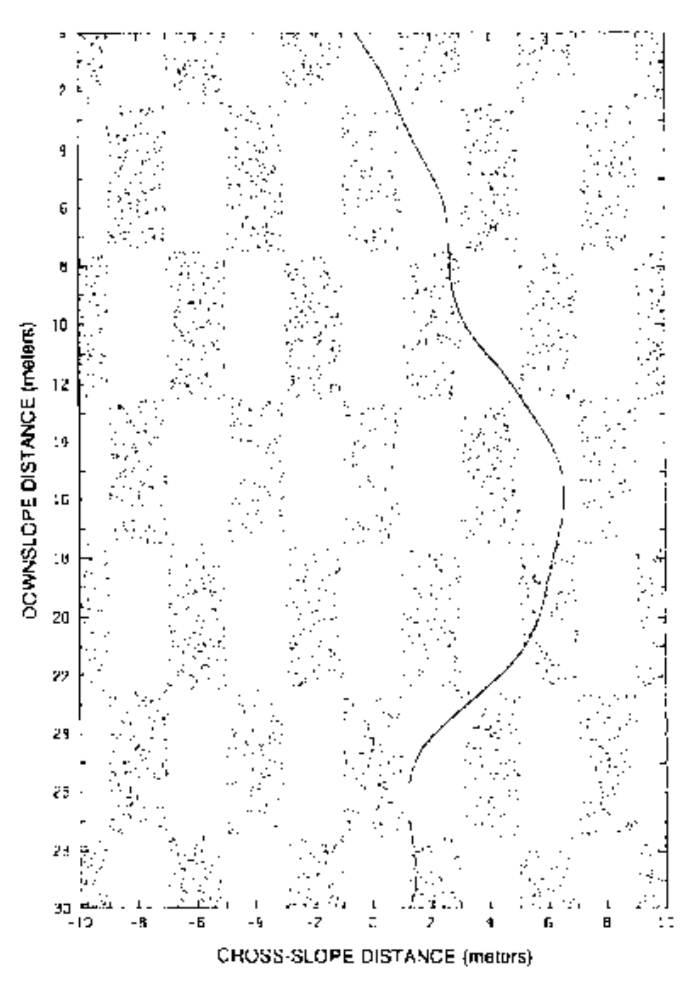
\includegraphics[height = 0.9\textheight]{figures/lorenz_essence_1993_fig6}}%
\only<3>{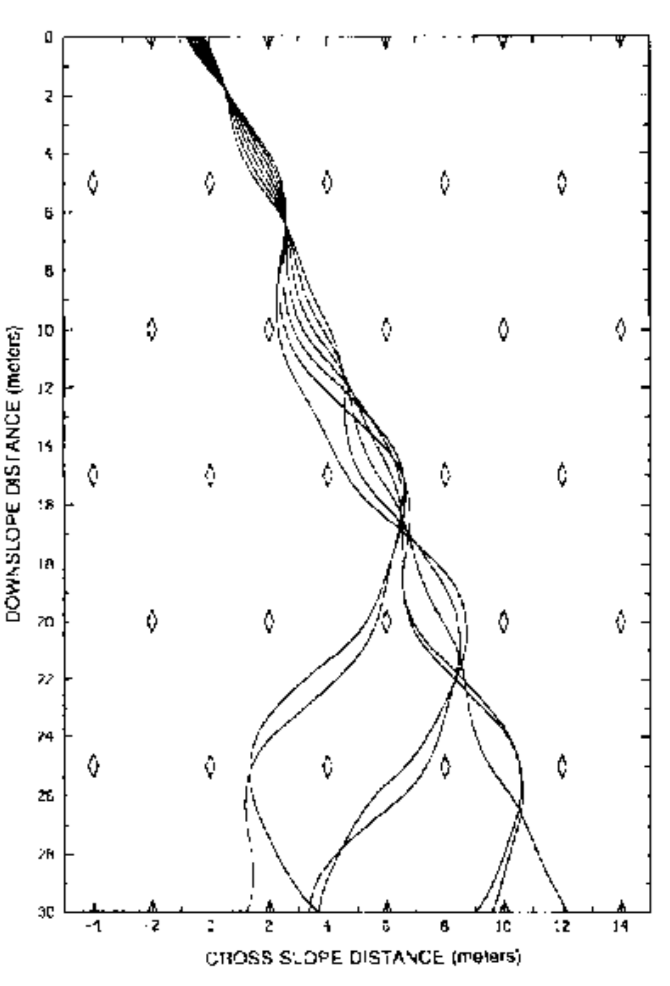
\includegraphics[height = 0.9\textheight]{figures/lorenz_essence_1993_fig7}}%
\only<4>{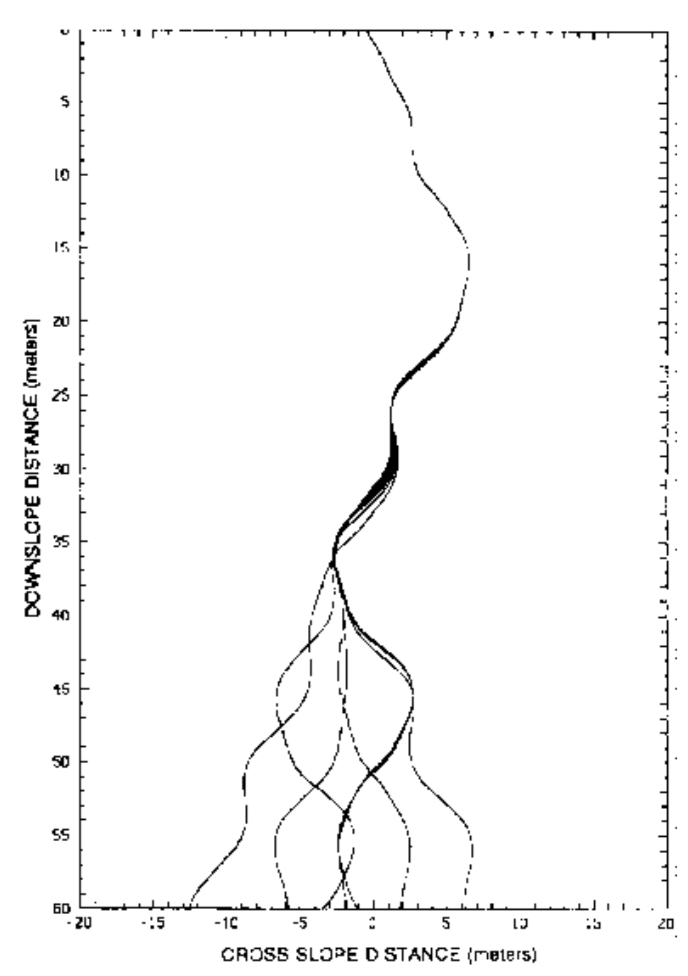
\includegraphics[height = 0.9\textheight]{figures/lorenz_essence_1993_fig8}}%
\end{center}

\end{frame}
%%%%%%%%%%%%%%%%%%%%%%%%%%%%%
\begin{frame}
\frametitle{}

\begin{center}
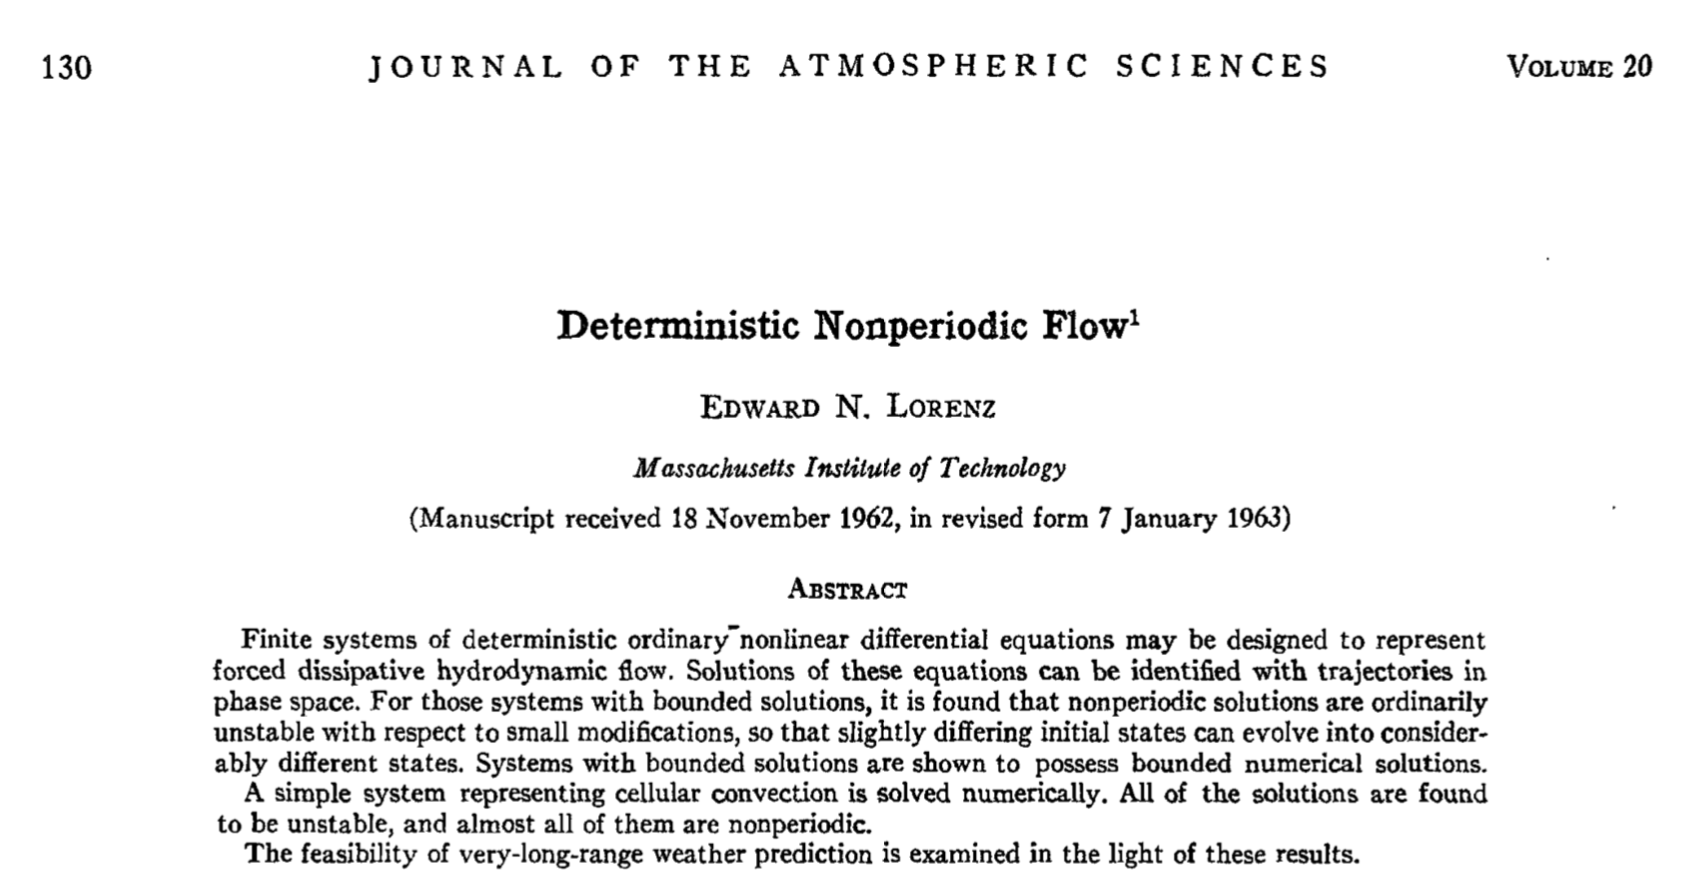
\includegraphics[width = 0.9\textwidth]{figures/lorenz_deterministic_1963_title_abstract}
\end{center}

\end{frame}
%%%%%%%%%%%%%%%%%%%%%%%%%%%%%%%
\begin{frame}
\frametitle{}

\begin{align*}
  x' &= \sigma(y-x) \\
  y' &= x(\rho-z)-y \\
  z' &= xy-\beta z
\end{align*}

\begin{itemize}
\item x: the rate of convective motion - i.e. how fast the rolls are rotating,
\item y: the temperature difference between the ascending and descending currents, and
\item z: the distortion (from linearity) of the vertical temperature profile.
\end{itemize}

\vfill
$\sigma = 10, \rho = 28,  \beta = 8/3$ 

\vfill
For more on how he came to study this system see Lorenz (1993) page 130 - 146

\end{frame}
%%%%%%%%%%%%%%%%%%%%%%%%%%%%%
\begin{frame}
\frametitle{}

\begin{align*}
  x' &= \sigma(y-x) \\
  y' &= x(\rho-z)-y \\
  z' &= xy-\beta z
\end{align*}

$\sigma = 10, \rho = 28,  \beta = 8/3$ 

\begin{center}
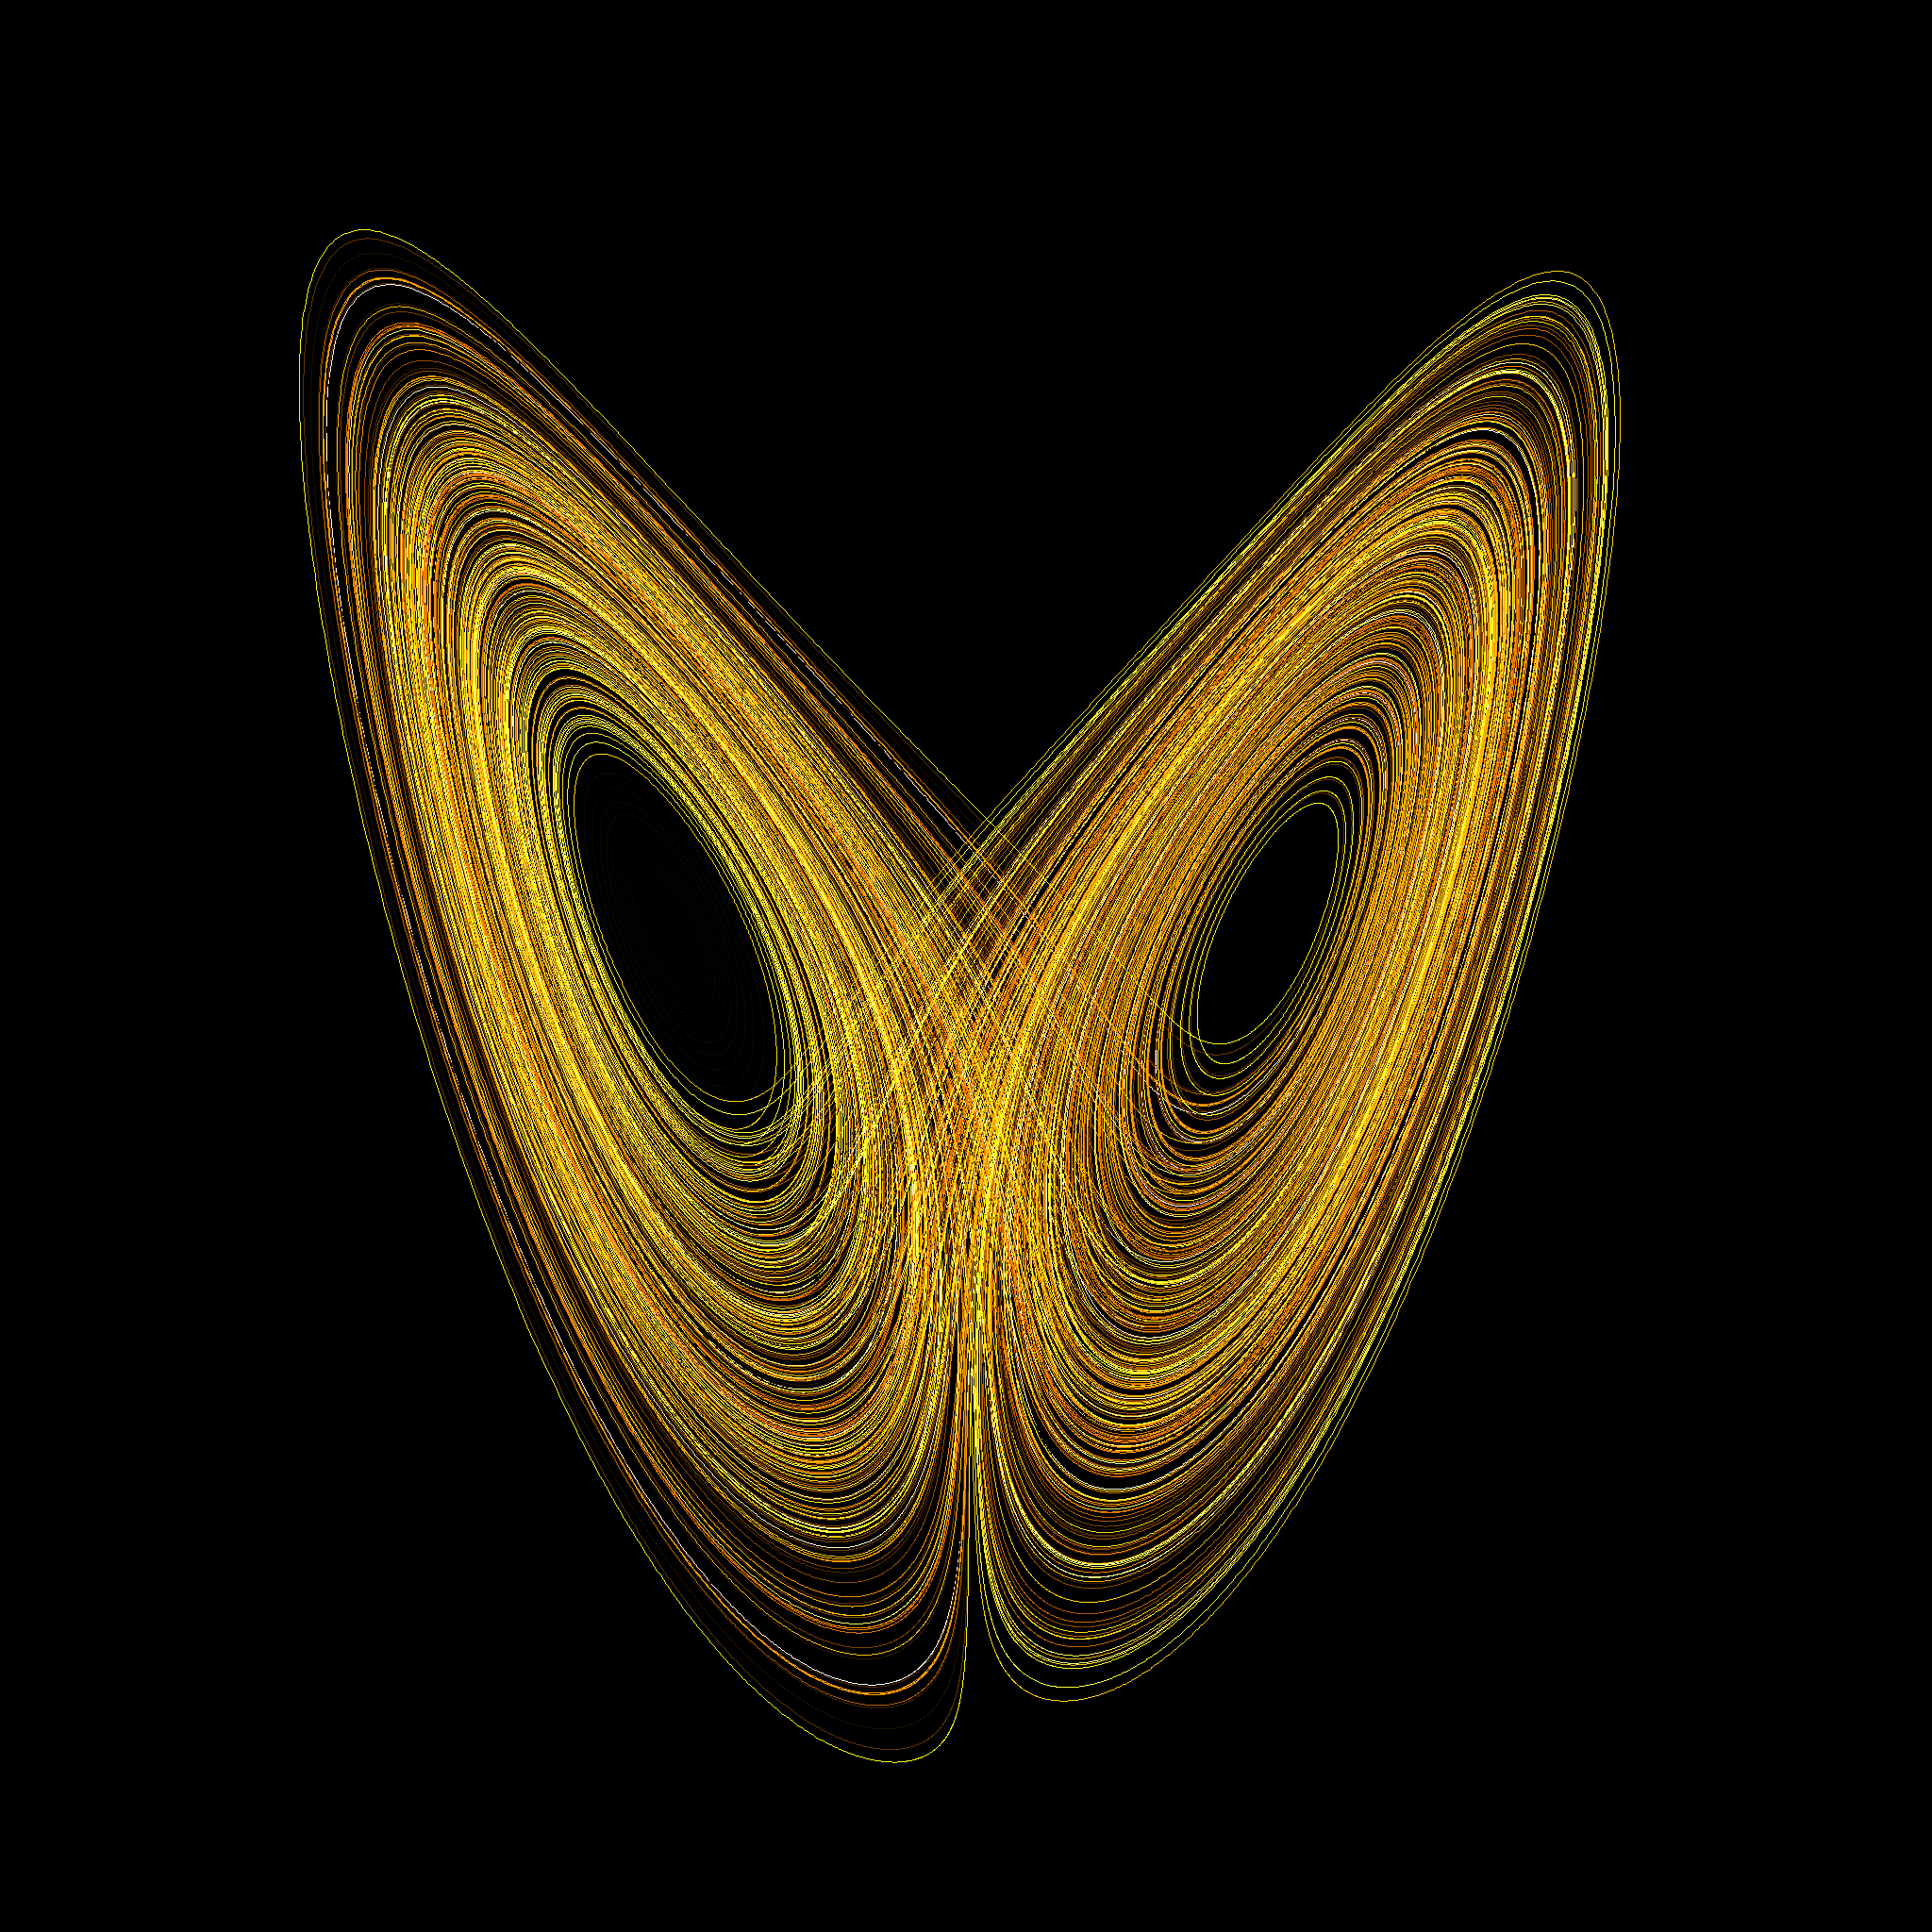
\includegraphics[width = 0.4\textwidth]{figures/Lorenz_system_r28_s10_b2-6666}
\end{center}

\vfill
\tiny{\url{https://commons.wikimedia.org/wiki/File:Lorenz_system_r28_s10_b2-6666.png}}
\end{frame}
%%%%%%%%%%%%%%%%%%%%%%%%%%%%%
\frame{\titlepage}


\end{document}
